\documentclass[12pt,a4paper]{article}
\usepackage{graphicx} 
\usepackage[utf8]{inputenc}
\usepackage[T1]{fontenc}
\usepackage[polish]{babel}
\usepackage{amsmath}
\usepackage{hyperref}
\usepackage{geometry}
\usepackage{float}
\geometry{a4paper, margin=2.5cm}

\title{\textbf{Założenia Projektowe: Program do wyznaczania GN}}
\author{Michał Majczek Bartosz Cynk}
\date{\today}

\begin{document}
	
	\maketitle
	
	\section{Cel Projektu}
	Celem projektu jest stworzenie wysokowydajnego, dwuwarstwowego systemu analitycznego do przetwarzania danych telekomunikacyjnych. System ma za zadanie automatyczną estymację Godziny Największego Ruchu (GNR) w sieciach komórkowych, co jest kluczowe dla procesu planowania pojemności sprzętowej. Głównym wymogiem niefunkcjonalnym jest portowalność -- system musi działać w środowisku Windows bez konieczności instalacji dodatkowego oprogramowania.
	
	\section{Założenia architektury}
	Projekt wykorzystuje architekturę grubego klienta z natywnym silnikiem obliczeniowym, implementując wzorzec separacji logiki od interfejsu użytkownika:
	\begin{itemize}
		\item \textbf{Interfejs Użytkownika:} Aplikacja odpowiada za interakcję z użytkownikiem, rysowanie wykresów słupkowych z dynamicznymi etykietami oraz zarządzanie procesami.
		\item \textbf{Silnik Obliczeniowy:} Natywna aplikacja konsolowa w języku \textbf{C++}. Uruchamiana asynchronicznie przez aplikację za pomocą CLI.
		\item \textbf{Baza Danych:} \textbf{SQLite}. Bezserwerowa baza plikowa, zapewniająca pełną przenośność i bezproblemowy zapis historii analiz.
		\item \textbf{Eksport Danych:} Metoda służąca do natywnego generowania raportów w formacie~\textbf{\textit{.xlsx} / JSON}.
	\end{itemize}
	
	\section{Algorytmy}
	Silnik analityczny (C++) przetwarza dane w granulacji 15-minutowej, implementując międzynarodowe standardy inżynierii ruchu (ITU-T):
	
	\subsection{TCBH (Time Consistent Busy Hour)}
	Wyznacza jedną, spójną czasowo godzinę szczytu dla całego badanego okresu. Algorytm uśrednia ruch w identycznych oknach czasowych w każdym z badanych dni. Zdefiniowany jest wzorem:
	$$TCBH = \max_{t} \left( \frac{1}{N} \sum_{i=1}^{N} X(i, t) \right)$$
	gdzie $X(i, t)$ to natężenie ruchu w dniu $i$ dla przedziału czasowego $t$, a $N$ to całkowita liczba dni.
	
	\subsection{ADPQH (Average of the Daily Peak Quarter Hour)}
	Metoda ,,ruchomego szczytu'', identyfikująca maksymalne obciążenie dla każdego dnia niezależnie, z dokładnością do przesuwanego okna 15-minutowego. Pozwala na precyzyjne śledzenie nieregularnych wahań ruchu:
	$$ADPQH = \frac{1}{N} \sum_{i=1}^{N} \max_{t_{15}} X(i, t_{15})$$
	gdzie maksymalizacja przebiega po wszystkich 15-minutowych interwałach danego dnia~$i$.
	\section{Projekt graficzny}
	\begin{figure}[H]
		\centering
		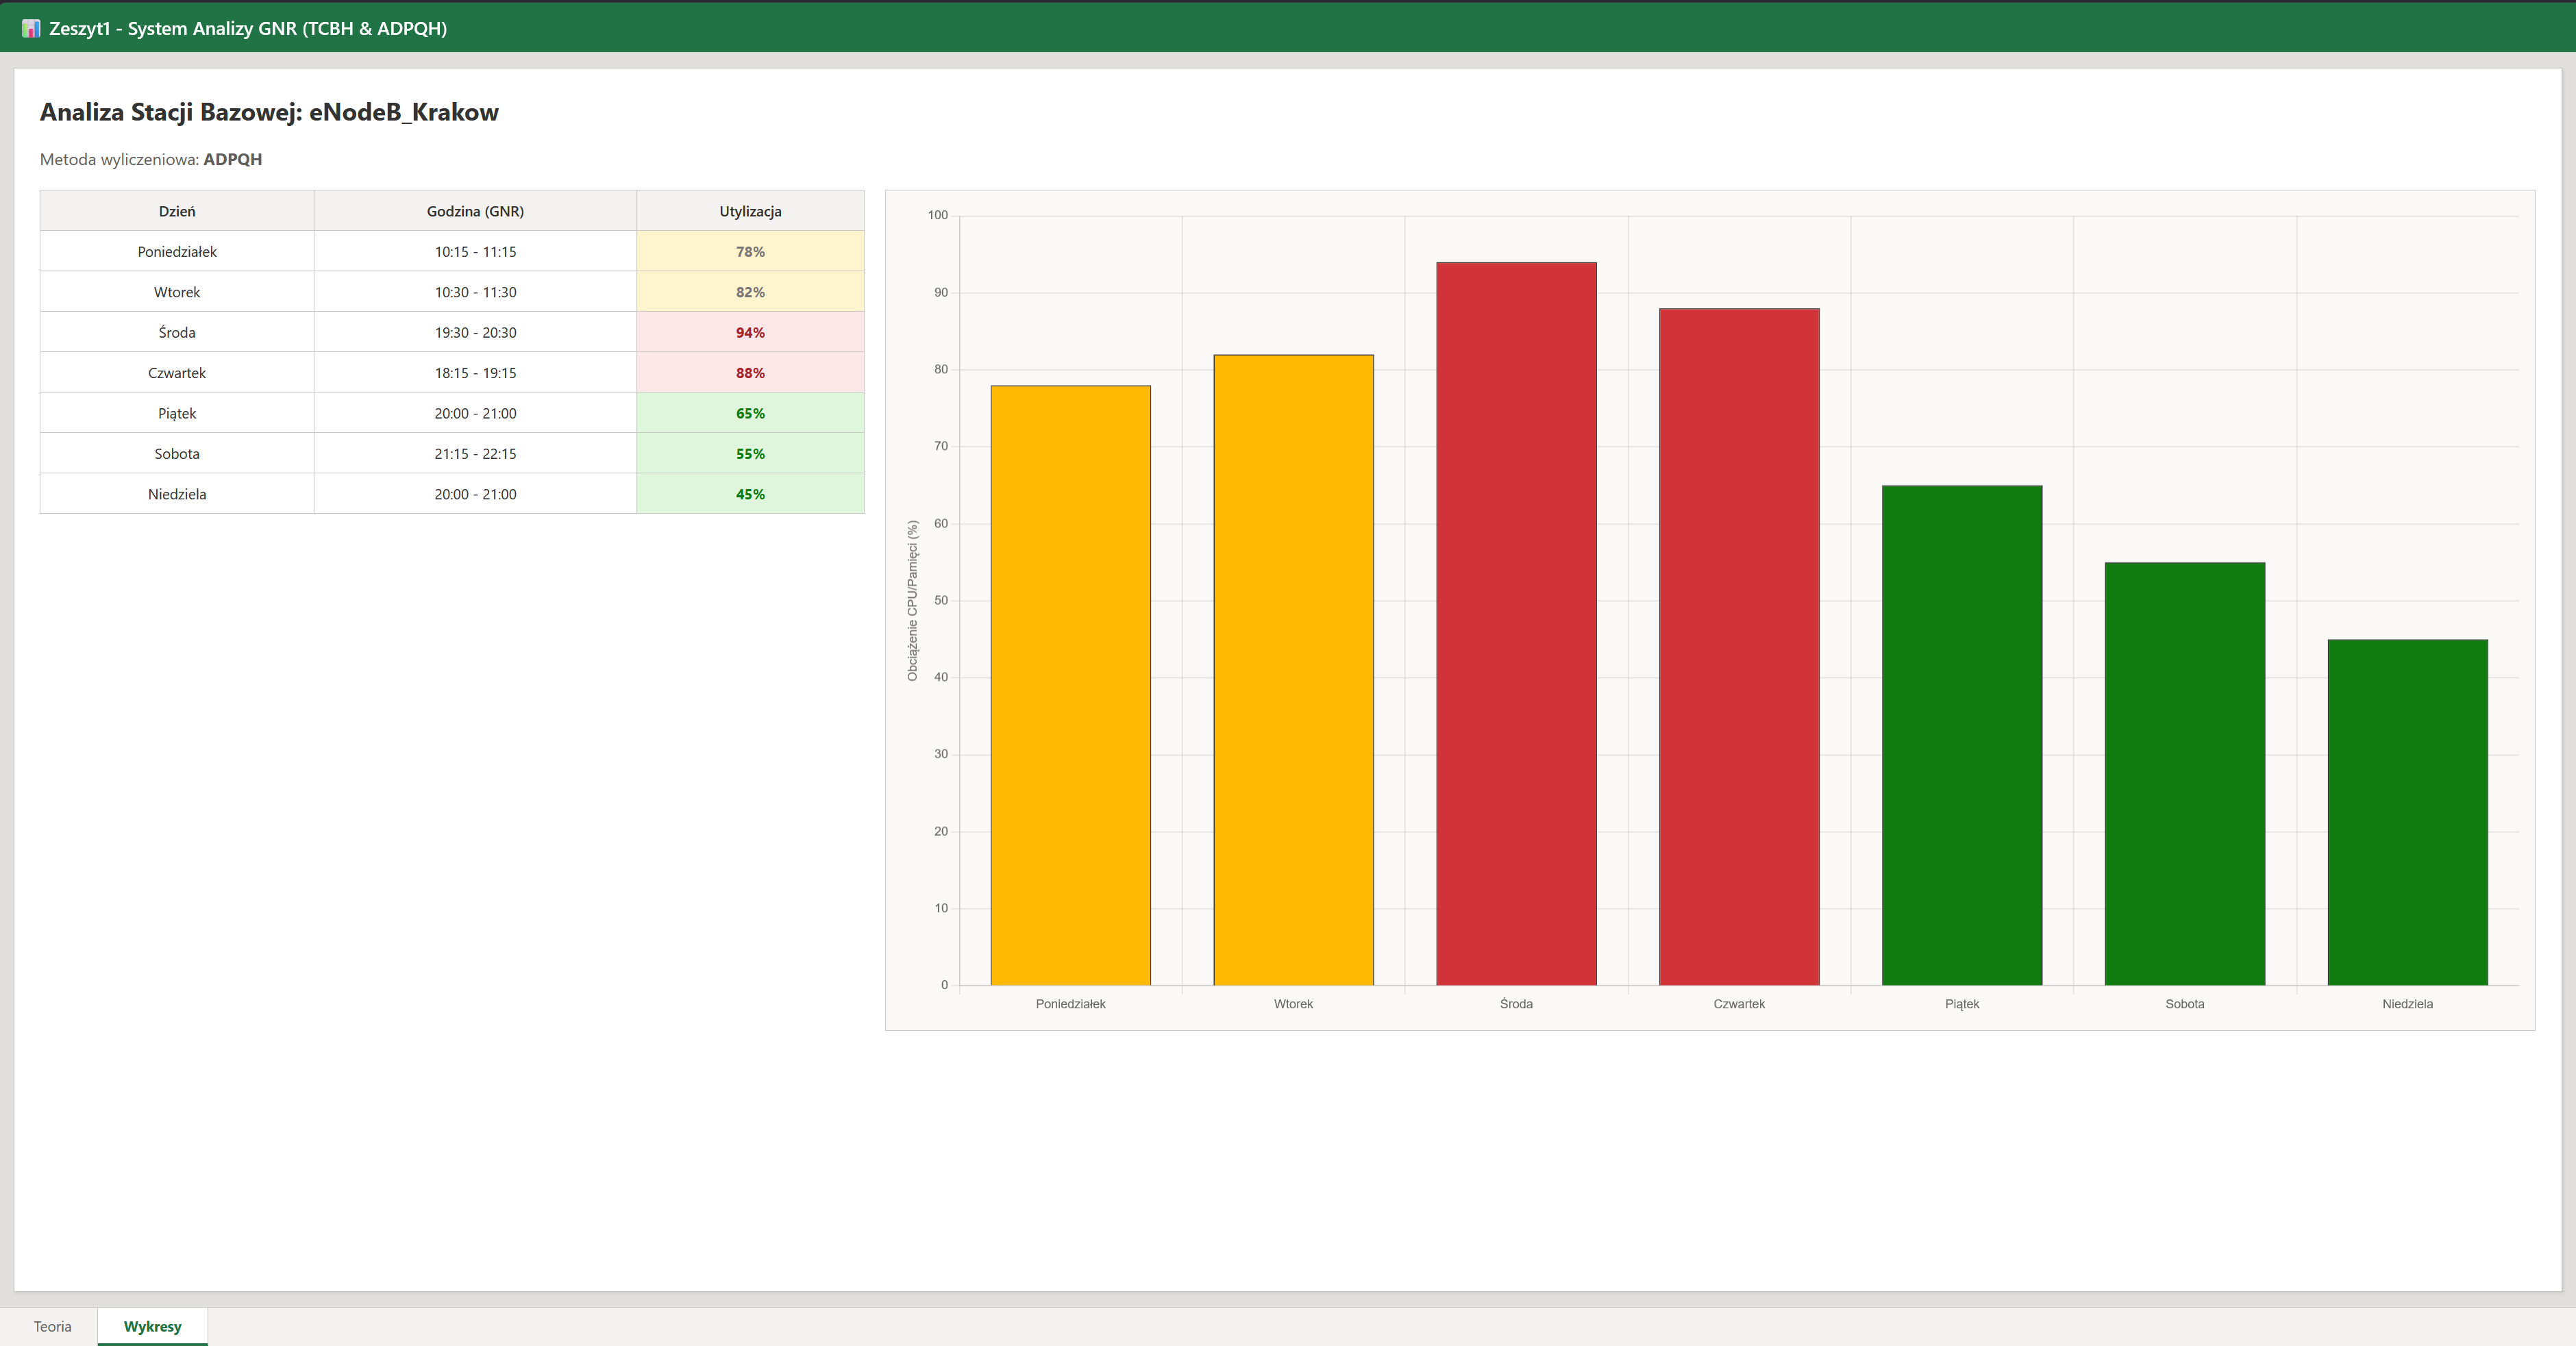
\includegraphics[width=0.9\linewidth]{koncept1}
		\caption{}
		\label{fig:koncept1}
	\end{figure}
	\begin{figure}[H]
		\centering
		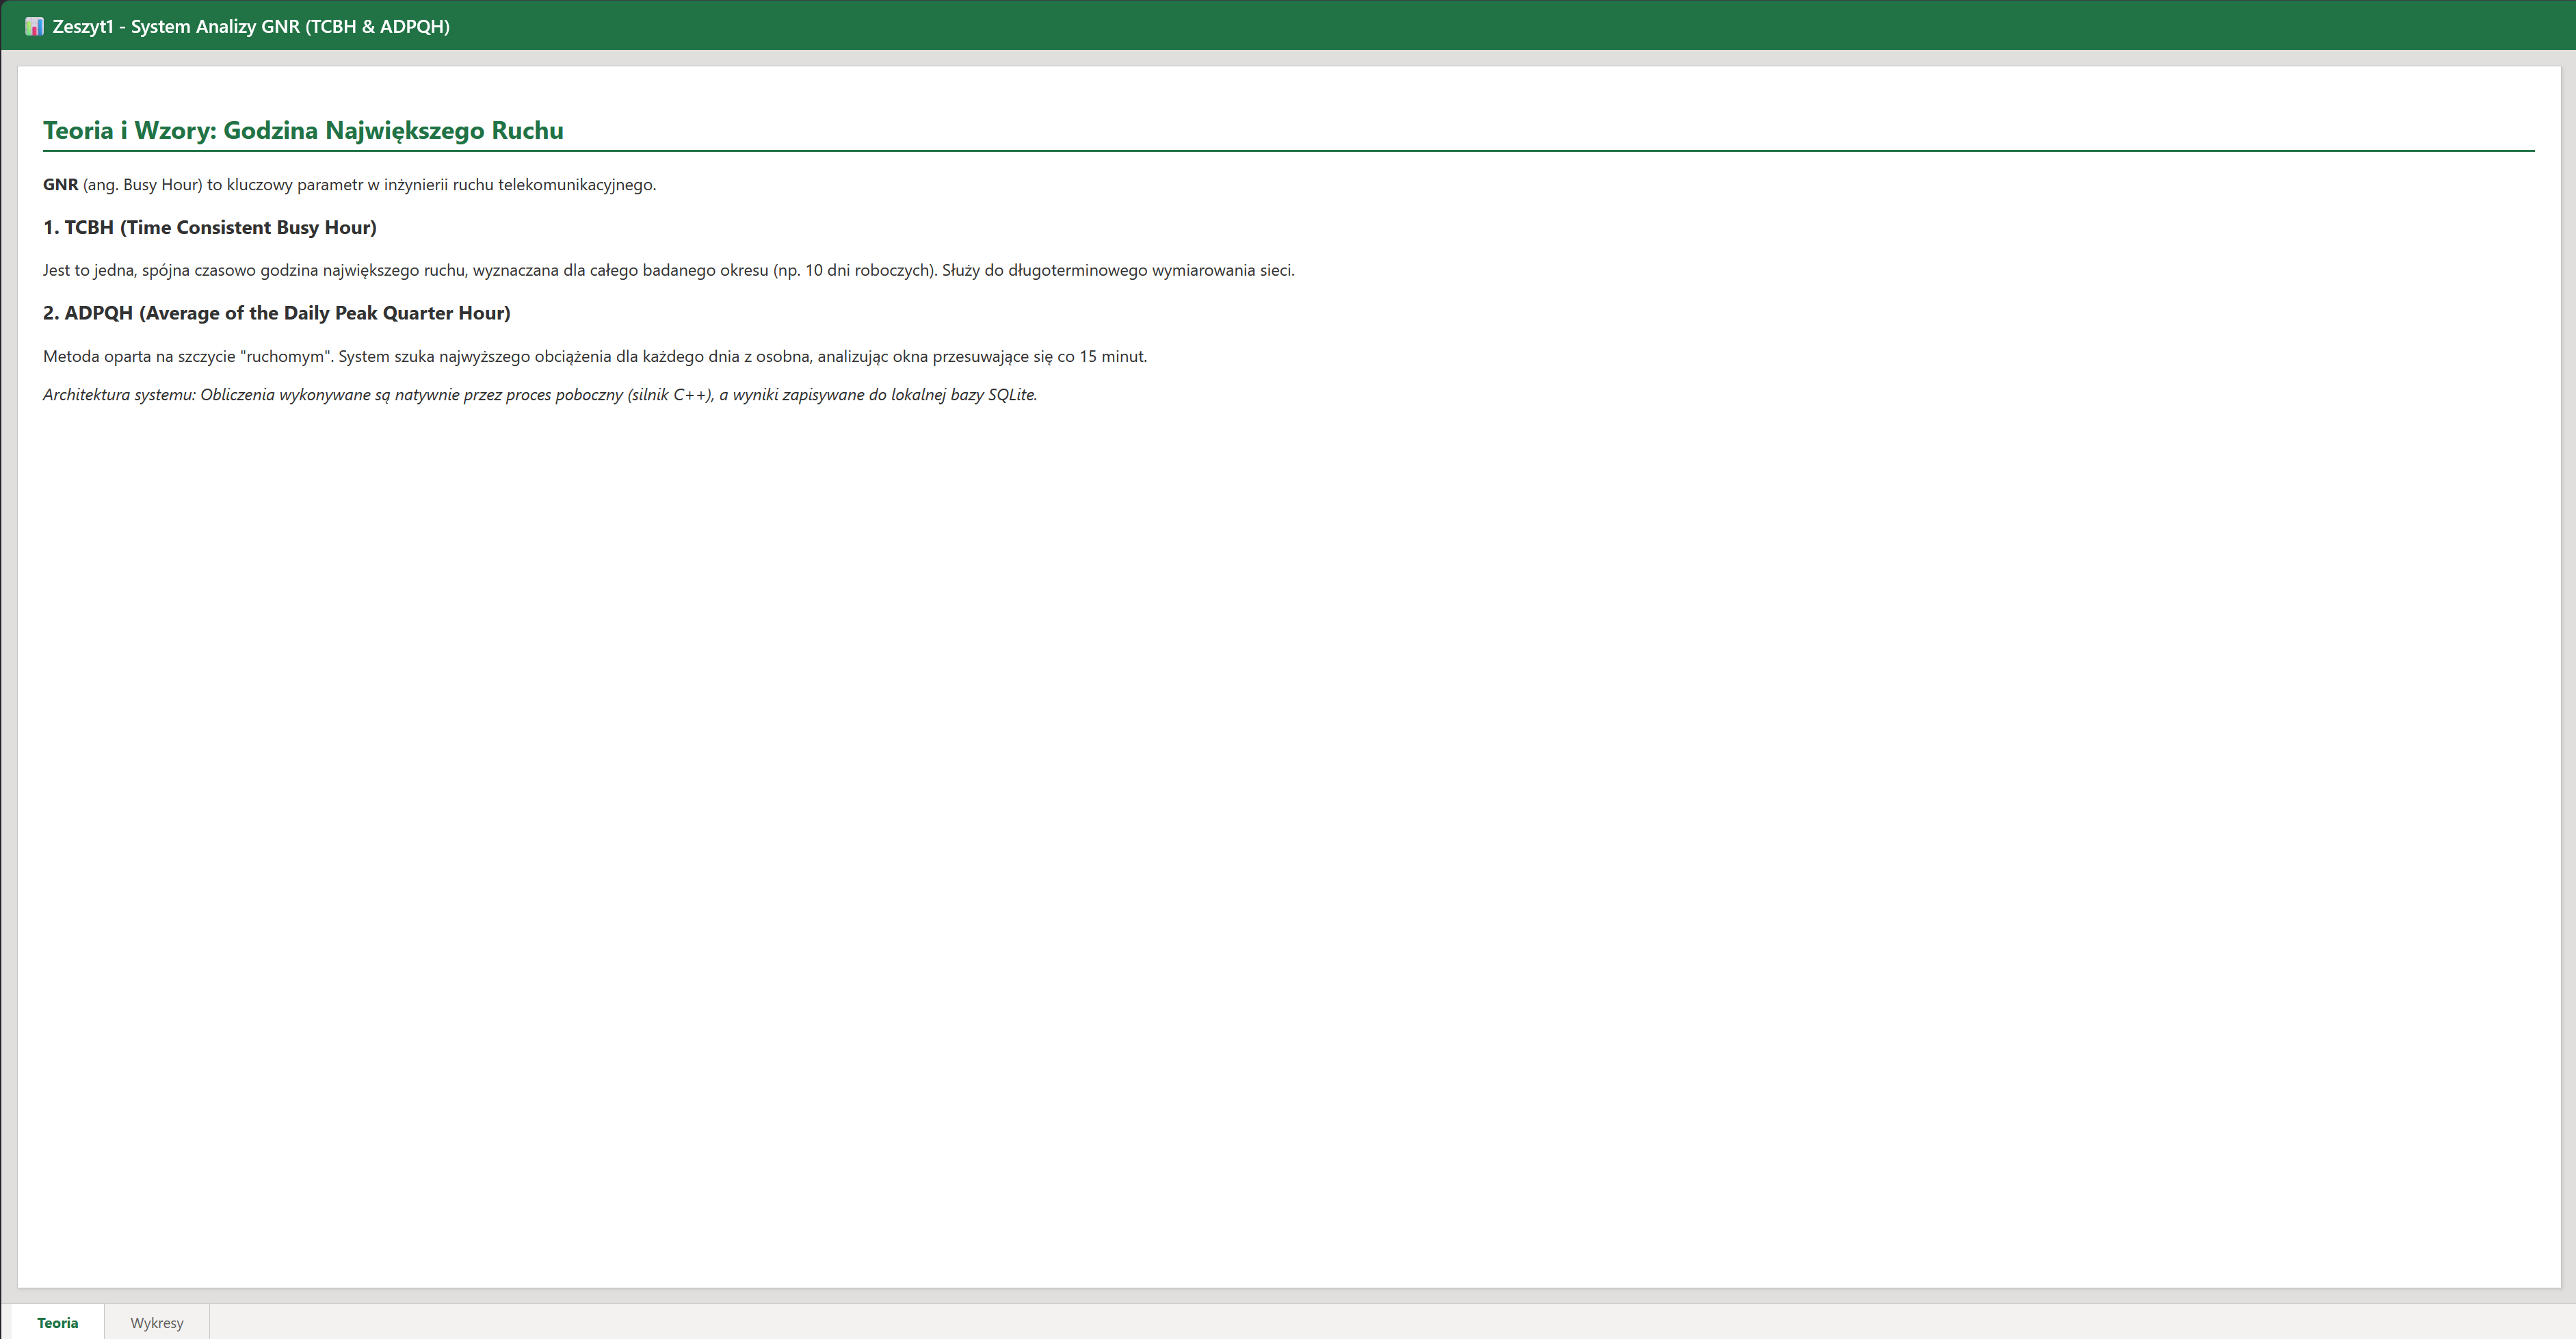
\includegraphics[width=0.9\linewidth]{koncept2}
		\caption{}
		\label{fig:koncept2}
	\end{figure}	


	\section{Struktura Wdrożeniowa}
	System dostarczany jest w formie pojedynczego katalogu, gotowego do uruchomienia z zewnętrznego nośnika pamięci. Katalog zawiera:
	\begin{enumerate}
		\item Przenośne środowisko.
		\item Skompilowany plik wykonalny silnika (\textit{silnik.exe}).
		\item Skompilowany plik wykonywalny / archiwum interfejsu.
		\item Automatycznie generowany plik bazy danych SQLite.
		\item Skrypt rozruchowy (\textit{START.bat}), uruchamiający całość jednym kliknięciem.
	\end{enumerate}
	
\end{document}